\documentclass[oribibl]{llncs2e/llncs}
\usepackage{geometry}                % See geometry.pdf to learn the layout options. There are lots.
\geometry{letterpaper}                   % ... or a4paper or a5paper or ... 
%\geometry{landscape}                % Activate for for rotated page geometry
%\usepackage[parfill]{parskip}    % Activate to begin paragraphs with an empty line rather than an indent
\usepackage{amssymb,amsmath}
\usepackage{graphicx}
\usepackage{amssymb}
\usepackage{epstopdf}
\DeclareGraphicsRule{.tif}{png}{.png}{`convert #1 `dirname #1`/`basename #1 .tif`.png}

\graphicspath{{WarpTask/figures/}{Res/figures/}} %do not forget the / at the end
%\include{{llncs2e}}

\title{Very Large Integer  and polynomial inner product}
\author{Timoth\'ee Ewart\inst{1}, Andreas Hehn$^2$, Matthias Troyer\inst{2} and Thierry Giamarchi\inst{1}}

\institute{Universit\'e de Gen\`eve, \email{timothee.ewart@gmail.com} \thanks{Thank you : Maxim Milakov, Peter Messmer  - NVIDIA, and  Williams Sawyer, Gilles Fourestey - CSCS}  \and Eidgen\"ossische Technische Hochschule Z\"urich }

%\date{}                                           % Activate to display a given date or no dater
\begin{document}
\maketitle
%\section{}
%\subsection{}
%\vspace{-0.65cm}
\begin{abstract}
The main purpose of the  VLI C++ library is to perform large integer arithmetic and  inner product of polynomial. Based on meta-programming and  hybrid (CPU/GPU) mode, it performs inner product, where polynomials have  one to four variables  up to order fourteen. The coefficients are represented  by large integer of 128 to 256 bits.  In this paper, we remember the basics of the inner product with polynomials, and  the assembly implementation of the  library. Then, we focus on the gpu implementation of the inner product.  All these algorithms are based on brute force attacks, as the size of the  problem should not justify a FFT approach. We save a factor up to 10 on CPU and 60 on GPU compared to a GMP solution.
\end{abstract}
\section{Introduction}
 A few libraries  LINBOX or NTL  deliver high performance in polynomial solvers.
These libraries are usually connect ed with GMP\footnote{GMP is the standard library for long arithmetic, gmplib.org} when needed. 
The introduction of hardware accelerator in HPC a few years ago and more recently GPU  by Nvidia introduce a revolution. It necessitates to adapt library to these new hardwares. 
The most famous example on this transition in mathematic is the famous blas/lapack libraries to MAGMA \cite{magma}, on the other side, polynomials libraries does not make the transition to GPU.
During the last few years, authors like \cite{Govindaraju2008, Emeliyanenko:2009, Moreno2010}, wrote polynomial multiplication  to  this new hardware, successfully. All these authors focus on large polynomials,
 with a FFT approach. 

In the present work, we are focusing on the inner product with dense and triangular multivariable polynomials.  The coefficients of the polynomials are large integer. 
We preferred develop a long integer library  han utilize GMP, because GMP is a dynamic library.
Moreover, we want a library natively compatible with GPU to allow hybrid calculation. GPU imposes contiguous memory which is impossible with a GMP approach.
Thus, we propose a static library based on contiguous memory where the exact assembly kernels are generated by meta-programming during the compilation, at the time, for CPU and GPU.
We do not wast time in the dynamic memory allocation and let the compiler optimizes deeply the library for both architectures.

\section{Polynomial and Inner product definitions}

The library performed inner product of vector of polynomials from one to four variables where polynomials are defined like (four variables) :
\begin{eqnarray}
P_a(x,y,z,w) & = & \sum_i^n \sum_j^n  \sum_k^n \sum_l^n  a_{ijkl} x^i y^j z^k w^l , \,\,\,\,\,\, \text{or} \\
                   & = & \sum_i^n \sum_j^{(n-i)} \sum_k^{(n-i-j)} \sum_l^{(n-i-j-k)}  a_{ijkl} x^i y^j z^k w^l  .
\end{eqnarray}
where  $x,\,y,\,z$ and $w$ are the variables,  $i,\,j,\,k$ and $l$  the indices, $a$  the coefficients, and $n$ the order of the polynomial.
Theses polynomials are named dense and  triangular polynomial, respectively.  If now we consider two vectors of polynomials of the  same type of $m$ 
entries  $\boldsymbol{v}_1<P_a>$ and  $\boldsymbol{v}_2<P_b>$. The inner product  consists of the product 
of every entries  associated to a global reduction. 
 \begin{eqnarray}
 P_c = \sum_i^m \boldsymbol{v}_{1_i}<P_a>  \times  \boldsymbol{v}_{2_i}<P_b> \label{poly1} \label{InnerProduct}
\end{eqnarray}
where $\times$ indicates the multiplication between two polynomials. The multiplications occurs basic rules of polynomials multiplication. 
A final coefficient may be the sum of several coefficients (named contributions), resulting from the sum of several multiplications. These coefficients are the cross terms. 
The cross terms are not a problem for the cpu version, as a polynomial multiplication is done by a single thread but they are the bottleneck for the gpu version.
The number of coefficient for a dense and triangular polynomial are given by $(n+1)^{\kappa}$ and  $(\kappa+n-1)! / ( (\kappa-1)! n! )$, where $\kappa$ is the number of variable. 

In term of  programming and parallelization, at least for the cpu version, the previous equations can be reduced by independent loops with a final reduction.
 These work can be easily done in OpenMP. Every OpenMP threads calculate several  polynomial multiplications and make a local reduction. At the end, a final reduction is performed  by the main thread.
 % \footnote{In OpenMP reduction for class is not supported}. Results showed a perfect scalability of the OpenMP code. 

\section{VLI  CPU library}

The coefficients of the polynomial are represented by a large integer named VLI number.  A VLI number is characterized by a size in bits; it is a  template parameter.
The size varies from 128 to 512 bits.  Its implementation is static, contrary to the well know GMP. 
Inside the memory, the VLI numbers are  contiguous. The data type container is an 64 bits unsigned integer array.

The basic operations supported by VLI are the four basic operations : $+,-,\times, /$, extended multiplications and bit shift operations. The library allows  operations between operands of the same type, and  integer. For performance issue, we have a specific solver for every operations except  the divisions. All the algorithms and operations are based on the childhood methods but the realizations has been done in assembly,
because, the assembly instructions facilitate the implementation and boost the performances.

\subsection{Assembly}

As we need carry\footnote{ The carry bit is a bit of the status register, as the overflow bit, 
it informs  the overflow of an operation, but it can be re-use to propagate the carry. } for addition/subtraction and an extended multiplication for the multiplication.
Although the hardware supports them; we can not access to these features by the C++ language, the only possibility is the assembly.

In assembly, these features  are supported by the pairs of mnemonic; \texttt{addq/adcq} for the addition; \texttt{sbbq/subq} for the subtraction and \texttt{mul} for the extentend multiplication.   
Combining these mnemonic, we reproduce easily long arithmetic algorithm. The ASM work is based on \cite{Hyde:2003:AAL:861534}. 

We coded the assembly using the GNU inline assembly, it consists of a string between ASM tag.
Generate by hand all these  assembly strings (kernels)  can be painful and a source of error \footnote{The library has near 8000 lines of assembly cumulated between x86-64, Power64, and PTX} 
We designed a generator of assembly. It creates, all versions of a kernels during the compilation.   
It is built on the boost preprocessor package, because we can create, manipulate the strings during the pre-compilation, 
and generate a specific tuned kernel for every large integer. All kernels use this procedure except the extended multiplication for the cpu.

The x86-64 architecture allows 16 registers (32 for power), as much as possible, we conserved the datas into the registers when we perform a long multiplication to reduce read/write actions to the
stack to the minimum. Additional optimizations have been done like full unrolling and assembly tips. We  supported  x86-64, Power64 and PTX (GPU) assembly.
Moreover GPU  assembly has specificities, it does not support carry bit for 64 bits integer, but only for 32 bits integer\footnote{Introduce since CUDA 4.2}.  
It allows multiplication-add 32 bits integers operations with carry bit support \cite{CUDAasm}. 
Work in 32 bits mode imposes twice more operations for the additions/substractions and one order of magnitude more for the multiplications. 

\subsection{Memory layout and SIMD implementation}

It exists at least two data layouts for this problem: the array of structure (AoS) and structure of array (SoA), both have  advantages and disadvantages. In our problem the AoS consists of saving the data in this order  : VLI - Series of VLI (polynomial coefficient)- series of polynomial (the vector). The SoA structure interleaves the coefficients of the VLI and the polynomials:
\begin{figure}
\begin{minipage}{0.50\linewidth}
\begin{eqnarray}
\tiny{
 \underbrace{
 \underbrace{ \underbrace{a^0_{00} | a^1_{00} | a^2_{00}}_{VLI, a_{00} } || \underbrace{a^0_{10} | a^1_{10} | a^2_{10}}_{VLI, a_{10}} ||   \dots  }_{1^{st} \textrm{polynomial}} 
      |||    \underbrace{ \underbrace{b^0_{00} | a^1_{00} | b^2_{00}}_{VLI, b_{00} } || \underbrace{b^0_{10} | b^1_{10} | b^2_{10}}_{VLI, b_{10}} ||   \dots  }_{2^{nd} \textrm{polynomial} } }_{\textrm{Vector of polynomial, AoS order}} \nonumber
}
\end{eqnarray}
\end{minipage}
\begin{minipage}{0.50\linewidth}
\begin{eqnarray}
\tiny{
 \underbrace{
 \underbrace{a^0_{00} | a^0_{10} | \dots || a^1_{00} | a^1_{10} | \dots  }_{1st  \textrm{ nested VLI/Polynomial} } |||  \underbrace{b^0_{00} | b^0_{10} | \dots || b^1_{00} | b^1_{10} | \dots  }_{2nd  \textrm{ nested VLI/Polynomial} }
 }_{\textrm{Vector of polynomial, SoA Order}} \nonumber }
\end{eqnarray}
\end{minipage}
\caption{Representation of the AoS Order (left) or SoA Order (right) for a vector of polynomial \label{AOSSOA}}
\end{figure}

The choice of the memory layout is important. It facilitates  the usage of the SIMD/AVX instructions. We choose the AoS for the following reasons:
we want reuse the VLI library in other object conception code, so we can not interleave the VLI number with the polynomial. 
The data structure should only concern the very large coefficient. Apply SIMD on AoS, for an addition it is a non sense because there is no specific instruction to propagate carry between entries of the multimedia register.
The extended multiplication under AVX \texttt{\_\_mm256\_mul\_epu32}  allows only four multiplication of 32 bits, we save a factor two. Nevertheless, on Sandy Bridge, we have 3 ALU, we can not exclude
the execution of several long multiplication in the same time, and we could loose the benefice of the SIMD version. Moreover, a large extra work is necessary to prepare the registers and shuffle the data which is expensive. For our range of operations the extended multiplication varies from 128 to 512 bits, a SIMD version will be not the optimum solution. Though, it has been used with success for larg integer ($>$1024 bits) \cite{SIMD}.

\section{A Short introduction to GPU}

A Graphical Portable Unit  is efficient  to address problems that can be expressed as data-parallel computations � the same program 
is executed on many data elements in parallel. Successful usage of GPU in HPC necessitates a good understanding of their design to reach great performance. A GPU is composed 
of several independent calculation  entities named streaming multiprocessors (SMs typically a tenth), where the SMs run hundreds of threads concurrently (typically 256) by group of 32 (warp).
The GPU programming model imposes to divide the problem into coarse sub-problem that can be solved independently in parallel by blocks of threads,
 and each sub-problem into finer pieces that can be solved cooperatively in parallel by all threads within the block. 
% During the execution, independent blocks will be executed on free SMs, where the program of the block is executed over the threads concurrently way.

In terms of memory all SMs  share  a large  memory (several GigaBytes) with  low performance; approximatively one hundred cycle for read/write operations.
Inside each SMs additional specials memories (constant, shared, texture, surface) are available. These memories are characterized by their behavior, they can be read only, shared, cache and more.  
They have still a common characteristic, a very high performance for read/write  operations in a few cycles only.
A good programming practice is to preload data from global memory to shared/texture at once, for subsequent computations.  \label{CUDA_PRACTICE}

Apply the GPU ideology on the polynomial inner product  means the polynomial multiplications will be execute in parallel on a SMs. Then a global reduction will sum all results polynomials. The division into blocks is natural, a block is a single entry of the vectors (equation \ref{InnerProduct}). All the difficultis consists of designing a parallel algorithm of the polynomial multiplication and the final reduction.

\subsection{Inner product booster on gpu}

\begin{figure}[t]
\begin{center}
\mbox{
\includegraphics[scale=0.37, angle=-90]{coeffs.eps} 
\includegraphics[scale=0.37, angle=-90]{warp.eps} 
}
\caption{Left: Results coefficients (red line) sorted in reverse order and group by warp. Right: Balance of the tasks over the warps.}
\label{algo_gpu}
\end{center}
\end{figure}

The first idea coming in mind: calculate every single multiplication per an independent gpu thread,  indeed for a  polynomial, the number of coefficient can be large and compatible with the number of SMs threads. Nevertheless,  the result coefficients may have several contributions. If the contributions are calculated by several threads, it necessitates reduction between threads. This solution introduces   synchronizations, and lower performance.
The peak performance will be reached, if the warps run the same amount of work, and every single thread into a warp should be responsible of the full contributions of an output coefficient.
To achieve this goal, we defined a task object. A task is a set of 32 result coefficients in a specific order. A task tells a  warp how calculates coefficient (the thread number one of the warp takes the first coefficient of the task and so on). The warps may not have the same number of tasks, as we equilibrate the workload.
We proceeded in two  steps; first on cpu, where a preliminary work is done, we prepare all informations on the tasks, and then, the calculation on GPU.

For the first step, we create a fictive resulting polynomial  represented by the indices and the contributions. They are sorted by descending order on the number of contribution
and group by 32 as a task. These tasks are reordered over the warps to equilibrate the amount of work. An illustration of this algorithm is illustrated on the figure \ref{algo_gpu}. 
More the polynomials will have coefficients  more the distribution of the tasks over the warps will be  uniform and the calculations will be efficient. 
We fix, the maximum number of warp to eight (8 warps - 256 threads), as far as possible, we assign at least two tasks per warps.
Thus, in function of the number of coefficients a warp may calculate one task, whereas an other warp may have several tasks to calculate.
 When the determination of the task's list is over,  we transfer  asynchronously the tasks lists in the global memory.
This method does not  change the order of the datas. As for the CPU version, we have an AoS order.
 \begin{table}[t] 
	\begin{center}
	 	\begin{tabular}{l l}
                           \hline 
                           \textbf{Task execution}  Algorithm &  \\ \hline
                           \begin{tabular}{c l l} 
                               \tiny{1:} & VLI tmp   &  $\vartriangleright$ Specific to every threads  \\
                               \tiny{2:} &  \textbf{for} over number of task list size &$\vartriangleright$  Depend of the warp \\
                               \tiny{3:} &  tmp $\,\, \wedge=$ tmp     & $\vartriangleright$ Flush to 0 \\    
                               \tiny{4:} &   VLI ResCoeff &$\vartriangleright$  Thread gets a result coefficient from a task \\
                               \tiny{5:} &  \hspace{0.2 cm}  \textbf{for} over the number of contribution  & $\vartriangleright$ Each thread loop over its coefficient  \\
                               \tiny{6:} &  \hspace{0.4 cm}   Indices$_i$ = GetIndices(ResCoeff) &$\vartriangleright$ Determine input indices \\
                               \tiny{7:} &  \hspace{0.4 cm}   tmp + = CoeffPoly$_1$(indices$_1$) $\times$ CoeffPoly$_2$(indices$_2$) &$\vartriangleright$ Perform the extended MulAdd  \\
                               \tiny{8:} &  \hspace{0.2 cm}   \textbf{end for} &\\
                               \tiny{9:} &  SaveSoA(tmp) & $\vartriangleright$ Write into the global memory under AoS \\                               
                               \tiny{10:} &  \textbf{end for} &\\                               
                          \end{tabular} &  \\ \hline
		 \end{tabular} 
		 \caption{Algorithm of the task execution on GPU for the polynomial multiplications. \label{ALGO}}
	\end{center}
\end{table} 

This task's list job is executed only once for all polynomial types,  we limit the overhead for the first inner product. As soon as,  all task's list are calculated, 
we transfer the datas of the polynomials asynchronously on the device (the global memory of the GPU is allocated once, we limit the workload of the cuda free/malloc),
 and the calculation of all polynomial multiplication start.
 
 First, both input polynomials  are cached into the texture memory. 
 %faster memory (shared or texture) in function of there size. 
% we privileged  the texture memory on Kepler architecture. %, and the shared memory on the Fermi architecture.
When a polynomial multiplication begins,  every warp get corresponding tasks (at least one) from the task's list and loop over its number of task. Then,
the threads into a warp gets their respective output coefficients and iterate over the number of  contribution.
For every iteration over contribution, the threads determine the input coefficients, read the corresponding data in the fast memory and perform the arithmetic operations: a extended multiplication and an optional long addition (if the result coefficient has several contributions). The calculation of an output coefficient  are  done into fast memory (texture for the input data, and register for the intermediate result). 
When the loop over contribution terminates,  we transfer the coefficients into the an intermediate buffer in the global memory, but in SoA  order to prepare the final reduction. 
The reduction is done using the standard method of Nvidia \cite{CUDAReduction} to achieve the highest performance.

%  It can be both in the shared, one polynomial into the shared and the second one into the texture or two in the texture memory. 
%The determination of which  fast memory (shared or texture) is determined during the compilation. Thus we avoid if statement and probable sequentialization of the warps. 

To conclude, this  algorithm has the great advantage to work well with dense and sparse polynomials. The main difficult consists  to design an efficient function "GetIndices" that determine the contributions.
 We also developed an optional hybrid mode between CPU/GPU, this  technic is usual in GPU computing \cite{magma}. We split the inputs vectors of polynomials into two chucks of datas, execute concurrently on CPU and GPU. Only at the end, a synchronization during  the memory transfer is done  by the final reduction.

\section{Results}

\begin{figure}[t!]
\begin{center}
\mbox{
\hspace{-0.5cm}
\includegraphics[scale=0.37, angle=-90]{ME128.eps} 
\hspace{-0.4cm}
\includegraphics[scale=0.37, angle=-90]{MC128.eps} 
%\hspace{-0.4cm}
%\includegraphics[scale=0.25, angle=-90]{ME256.eps} 
}
\caption{Left: Dense polynomial inner product up to 3 variables with 128 to 256 bits coefficients. Right: Triangular polynomial inner product up to 4 variables with 128 to 256 bits coefficient. The 4 variables curves miss points due to not enough memory on the node. Larger coefficients give the same results.  Size of the vector 4096.}
\label{ResME}
\end{center}
\end{figure}

Benchmarks are performed on the facilities of The Swiss Center for Scientific Computing (CSCS), on cray  xk7 cluster for the GPU and a Sandy Bridge  node 32 logical cores  (HyperThreading on) Xeon E5-2670. The size of our vector is equal to 4096, the order of the polynomials varies from 1 to 14, the size of the inputs coefficients of the polynomials varies from 128 to 256 bits, the output polynomial has twice larger coefficients (256 to 512 bits). 

Evaluate  integer benchmarks integer are not easy, contrary to float number,  the integers operations are performed by ALU,  the number of  ALU  between processors, and the execution of the operations are  not constant \cite{ASMcost}.  We compute the  result  numbers as operations \footnote{A operation can be a long multiplication, addition and so on}   per seconds $GOP/s=10^{-9} \times batch/t$, where  $batch$ is the number of long integer operations computed during the execution (additions and multiplications), $t$ [s]  is the elapsed time, for more realistic comparison the execution time for GPU contains the memory  transfer. 

 The Figure \ref{ResME} presents the performance of a dense and triangular polynomials inner product. It compares our CPU library to GMP ( where polynomials are just instantiated with VLI or GMP),  we get an excellent speed up factor from 4 to 11. For two raisons, the coefficient of the  polynomial are allocated in the heap, in the case of GMP, they are allocated in the stack, it is well know better performances are obtained with less dynamic memory allocation.   The second raison, the meta-programming allows the construction of a specific solver for every type of large integer during the compilation, contrary to GMP, we do not have a universal solver (as GMP  for small size), the solver is unique with the maximum optimizations. % (operations are performing in the register only, no stack call).
  
The GPU curves show again an excellent speed up to factor 10 to 60 maximum compared to GMP, but with an interesting features. 
For both kind of polynomials, the performances for one variable are low, because we have a small number of threads during the execution of the GPU algorithms.
As the number of threads is fixed by the number of coefficient, $2n$ for a dense polynomial,  the maximum number of threads will be 28
 which corresponds to one warp. We do not utilize the capacity of the GPU. For two and more variables, whatever the polynomials, the performance are like a parabola. The position of the maximum is specific to the type of polynomial.  We obtained the maximum of performance, if the following conditions are respected. The number of running threads is maximum; 256 threads, and both inputs polynomials 
are cached into the texture memory. On Kepler the size of the texture memory is equal to 48 kB, this memory  is highly optimized for repetitive and random access contrary to shared memory
 (where bank memory conflict can appear).  Moreover, for large order, the result polynomial have  more coefficients, so the balance of the tasks over the warp is good, and consequently the efficiency too.
 

\begin{figure}[t!]
\begin{center}
\mbox{
\hspace{-0.5cm}
\includegraphics[scale=0.37, angle=-90]{ME128MIPS.eps} 
\hspace{-0.4cm}
\includegraphics[scale=0.37, angle=-90]{MC128MIPS.eps} 
%\hspace{-0.4cm}
%\includegraphics[scale=0.25, angle=-90]{ME256.eps} 
}
\caption{Dense and triangular polynomial inner product in [GIPS]. From 1 to 4 variables with 128 to 256 bits coefficients. Size of the vector 4096.}
\label{ResMEMIPS}
\end{center}
\end{figure}

For the small orders the number of GPU threads is lower than 256 but it will increase with the order until a maximum.
After, for the larger orders, although the number of threads is 256, the polynomials will be not full cache into the texture memory. So the execution kernels calls data from the global memory that reduce the performance.
 All this behavior show the difference between a CPU and a GPU. A CPU has really more transistor for the  data caching and flow control, it assures a regular and optimum access to the data. For the GPU,
 the programmer manages by hand the flow control, in return, it will have more transistor for the data processing, and consequently the performance.

Although translate the results into MIPS is hard, we did it, at least on GPU because the GPU kernel of the extended multiplication utilizes only one PTX instruction (\texttt{madc}).  Counting the total number of this  ASM instruction during 
the inner product, and dividing by the elapsed time, we obtain an estimation in GIPS (Giga Instruction Per Seconds). A  profiling of the code with CUDA profiler indicates the bottle neck of the application is the product of polynomial, so we do not take into account   the transfer of the data and the ASM instructions into the reduction. Therefore, we underestimate the performance of the library.
The peak performance of  a sample card based on Kepler GK110 is evaluated easily from CUDA documentation, for 32-bit integer multiply-add on 14 SMs * 700 MHz * 32 instructions per clock per SM = 314 GIPS. The results are reported in the figure \ref{ResMEMIPS}, we obtain 67\% of the Kepler card, that is a good result. The results are better for the dense polynomial because the coefficient \texttt{GetIndices} of the GPU algorithms is more time consuming for the triangular polynomials.

\section{Conclusions and future work}

The VLI library gives efficient solvers for the 128 to 512 bits integer associated to polynomial with 1 to 4 variables. We obtain a comfortable speed up until 60 compare to GMP for the our specific range. 
We aware the comparisons to GMP were not fair. GMP excels in thousand bits arithmetic, where our library can not work. As future work, we would like to implement, new kinds of polynomials, and a better management 
of  memory to maintain the performance of the inner product on GPU.

\bibliographystyle{llncs2e/splncs}
\bibliography{biblio/vlibib}


\end{document}  